\documentclass[11pt,a4paper]{article}
\usepackage[margin=2cm]{geometry}
\usepackage[T1]{fontenc}
\usepackage{lmodern,microtype,graphicx,booktabs,enumitem,xcolor,hyperref,titlesec,amsmath}
\usepackage[most]{tcolorbox}
\definecolor{navy}{HTML}{1D2F82}\definecolor{warn}{HTML}{C0392B}\definecolor{ok}{HTML}{2E8B57}
\hypersetup{colorlinks,linkcolor=navy,urlcolor=navy}
\titleformat{\section}{\Large\bfseries\color{navy}}{\thesection}{0.6em}{}
\titleformat{\subsection}{\large\bfseries\color{navy}}{\thesubsection}{0.5em}{}
\setlist{itemsep=2pt,topsep=3pt}
\graphicspath{{../figures/}{../diagrams/}}
\newtcolorbox{say}{colback=navy!4,colframe=navy,boxrule=0.6pt,arc=2pt,left=6pt,right=6pt,top=3pt,bottom=3pt,fonttitle=\bfseries,title=Say this}
\newtcolorbox{careful}{colback=warn!4,colframe=warn,boxrule=0.6pt,arc=2pt,left=6pt,right=6pt,top=3pt,bottom=3pt,fonttitle=\bfseries,title=Be careful}
\newcommand{\qa}[2]{\par\smallskip\noindent\textbf{Q: #1}\par\noindent\hspace*{1em}\begin{minipage}[t]{\dimexpr\linewidth-1em}#2\end{minipage}\par}

\title{\color{navy}\textbf{Review 2 Reading Guide \& Cheatsheet}\\[4pt]\large Design of a Temperature-Compensated PLL Frequency Synthesiser}
\author{For Viju Sanjai --- Review II, 30.09.2026}
\date{}
\begin{document}
\maketitle
\vspace{-1.5em}
\noindent This guide explains everything done between Review 1 and Review 2, why it was done, the numbers to know, and how to answer the hard questions. Every number here comes from \texttt{results/figdata.json} or \texttt{scripts/analyze\_mc.py}, the same data the slides use.

\tableofcontents
\newpage

%=====================================================================
\section{The story in 60 seconds}
\begin{say}
A ring-oscillator VCO changes frequency with temperature, so a PLL built around it has to work harder, or drop out of lock range, as the chip heats up. We built a complete integer-N charge-pump PLL in the open sky130 process and simulated it in ngspice. We measured the drift at all five process corners and found a 12.5$\times$ spread in temperature coefficient, not the 3.4$\times$ we reported in Review 1. We then designed a correction voltage that adds $k_1(T-27)+k_2(T-27)^2$ to the VCO control voltage. At the typical corner, the second-order version cuts the drift span from 8.51\% to 1.12\%. It meets our $\pm$0.3\% target only at the ff and sf corners. We validated the result at held-out temperatures and with a 30-sample Monte Carlo analysis using paired statistics. We also fixed the cold-start problem left open in Review 1: the loop now locks in 839 ns from 0 V.
\end{say}

\noindent\textbf{The three things Review 2 added}
\begin{enumerate}
\item \textbf{Characterisation:} the full 5-corner $\times$ 6-temperature VCO grid.
\item \textbf{Compensation:} 1st- and 2nd-order correction, fitted per corner and validated honestly.
\item \textbf{Robustness:} the cold-start fix, plus a Monte Carlo analysis with correct statistics.
\end{enumerate}

%=====================================================================
\section{The system: what each block does}
\begin{center}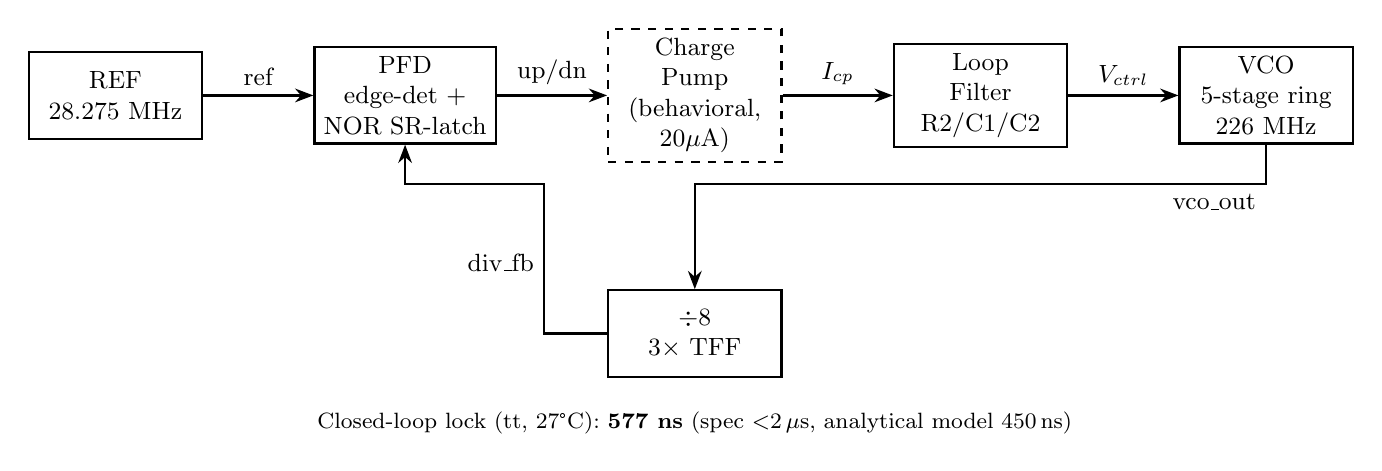
\includegraphics[width=\linewidth]{pll_block_diagram.png}\end{center}
\begin{itemize}
\item \textbf{Reference:} 28.275 MHz. The target output is $8\times$ that, $\approx$226 MHz.
\item \textbf{PFD (phase-frequency detector):} compares the reference edge against the divided VCO edge and outputs UP or DN pulses in proportion to the phase error. It is built from edge detectors and NOR SR-latches rather than resettable D flip-flops, because a reliable asynchronous reset fights the latch's own feedback.
\item \textbf{Charge pump:} converts UP/DN pulses into current pulses of $I_{cp}=20\,\mu$A into the loop filter. In Review 2 this is an idealised behavioural source; the transistor-level version is Review 3.
\item \textbf{Loop filter:} $R_2=1.7\,$k$\Omega$ in series with $C_1=68\,$pF, and $C_2=6.8\,$pF in parallel. It integrates the current into a control voltage $V_{ctrl}$. $R_2$ adds the zero that keeps the loop stable; $C_2$ smooths the ripple.
\item \textbf{VCO:} a 5-stage current-starved ring. $V_{ctrl}$ sets the starving current, which sets the delay per stage and therefore the frequency. $K_{VCO}\approx669$ MHz/V at 0.9 V. It stops oscillating below about 0.63 V.
\item \textbf{Divider $\div8$:} a chain of toggle flip-flops. It feeds the divided clock back to the PFD.
\end{itemize}

\begin{center}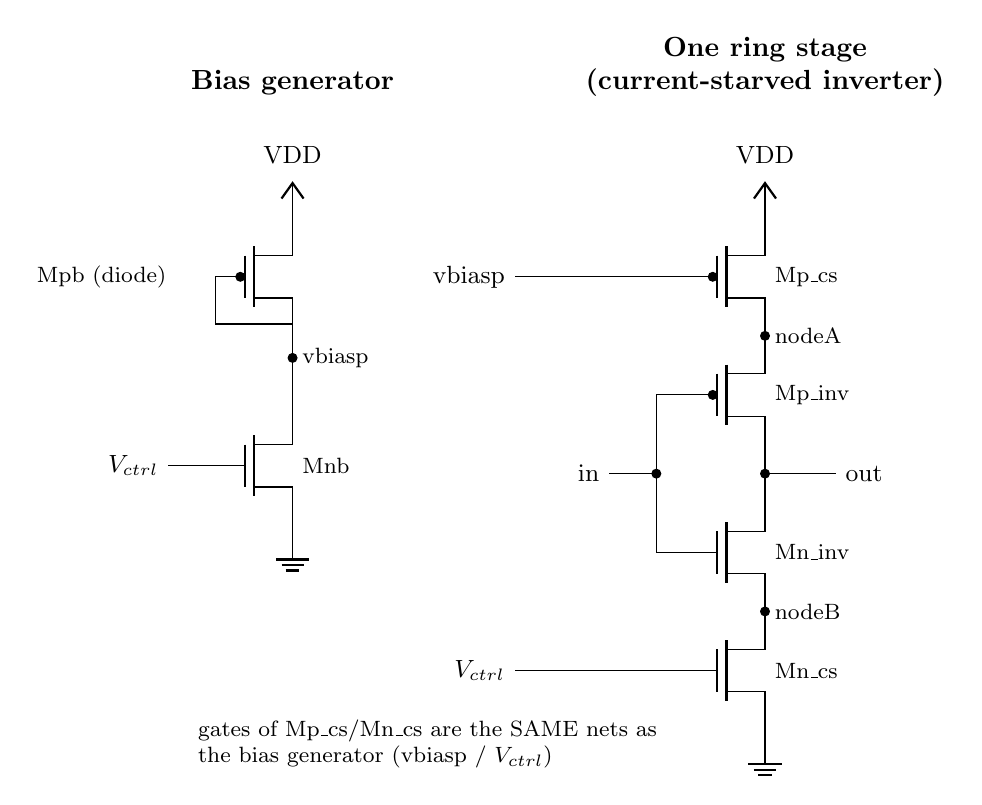
\includegraphics[width=0.5\linewidth]{vco_schematic.png}\hfill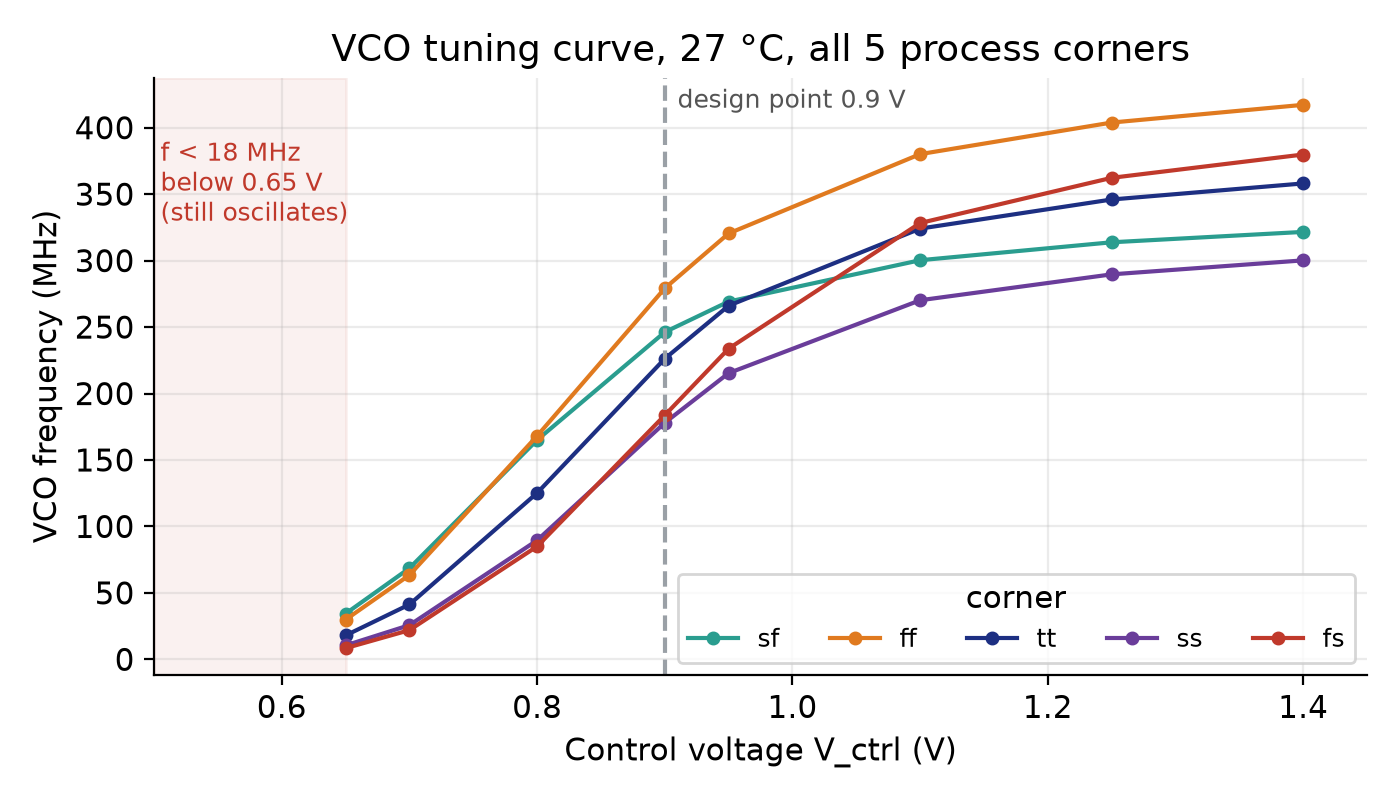
\includegraphics[width=0.48\linewidth]{tuning.png}\end{center}

\noindent\textbf{How to read the tuning curve.} The slope of this curve is $K_{VCO}$. At 0.9 V it is 669 MHz/V at tt, obtained from the derivative of a polynomial fit rather than a two-point secant. The flat region below 0.63 V is where the ring stops oscillating, and that is exactly why a cold start from 0 V was a problem.

%=====================================================================
\section{Result 1: uncompensated drift across all corners}
\begin{center}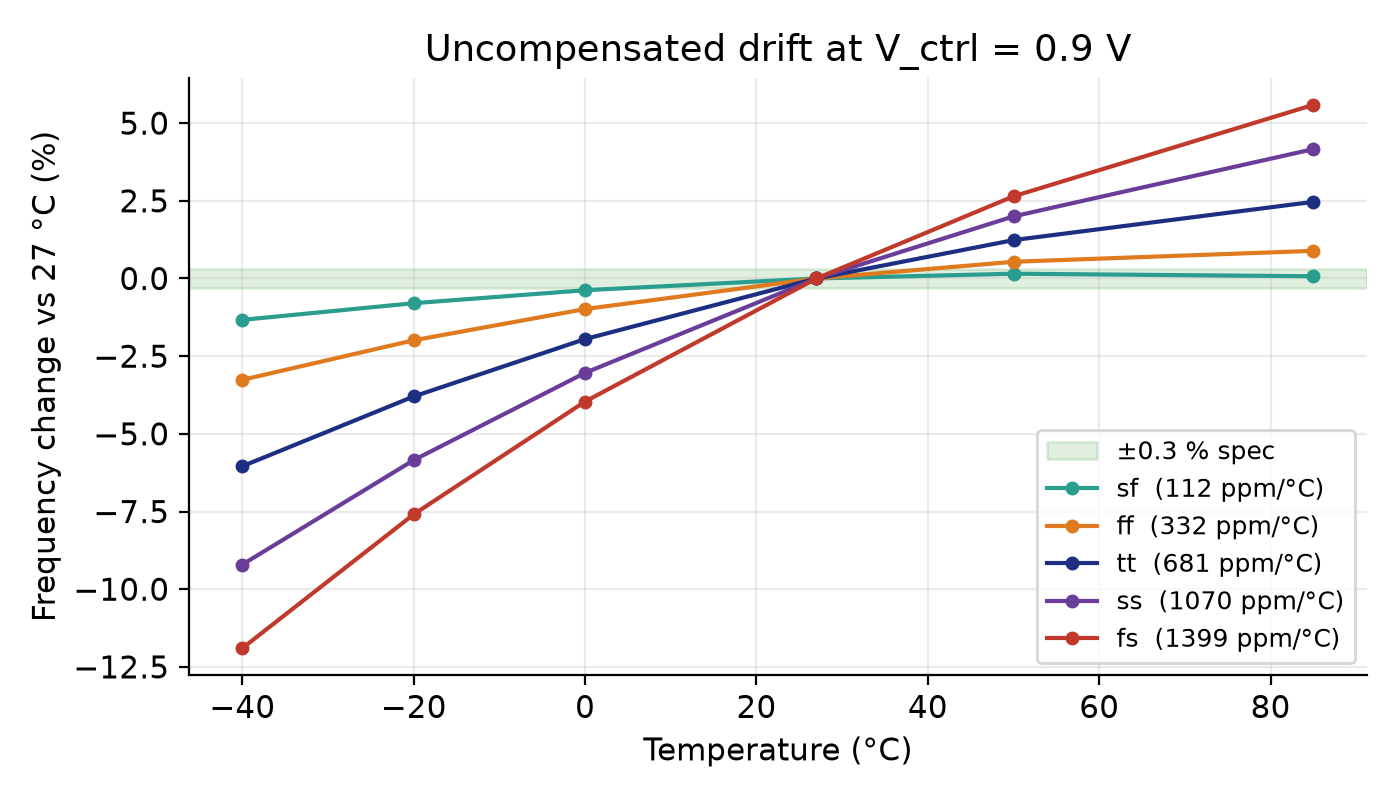
\includegraphics[width=0.62\linewidth]{drift_uncomp.png}\hfill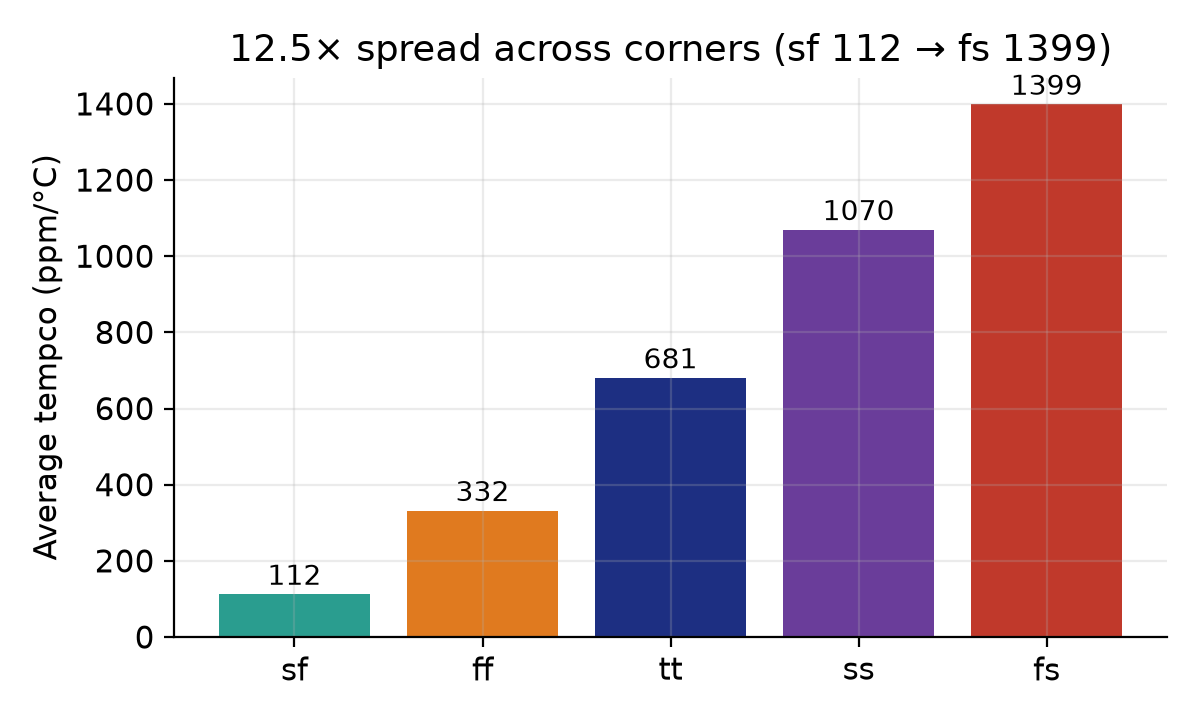
\includegraphics[width=0.36\linewidth]{tempco_bar.png}\end{center}
\begin{itemize}
\item \textbf{Procedure:} fix $V_{ctrl}=0.9$ V, sweep $T\in\{-40,-20,0,27,50,85\}$ \textdegree C, and do this at all 5 corners (30 simulations).
\item \textbf{Tempco} $=(f_{85}-f_{-40})/(f_{27}\cdot125)$ in ppm/\textdegree C. Values: sf 112, ff 332, tt 681, ss 1070, fs 1399.
\item \textbf{The correction to Review 1:} with only 3 corners we reported a 3.4$\times$ spread. The full grid shows 12.5$\times$, because fs, the worst corner, had never been simulated.
\item \textbf{Insight:} the \emph{mismatched} corners (sf, fs) bracket the range, not the matched ones (ss, ff). This suggests the balance between the NMOS and PMOS current sources drives the tempco, rather than raw device speed.
\end{itemize}
\begin{careful}
Frequency \emph{increases} with temperature here, the opposite of the textbook ``mobility falls, so the circuit slows down''. Our interpretation, which we have \emph{not} isolated by simulation: at this bias, the fall in threshold voltage with temperature outweighs the fall in mobility, so the starving current rises. If asked, present it as the likely mechanism, not a measured fact.
\end{careful}

%=====================================================================
\section{Why second order: the drift is curved}
\begin{center}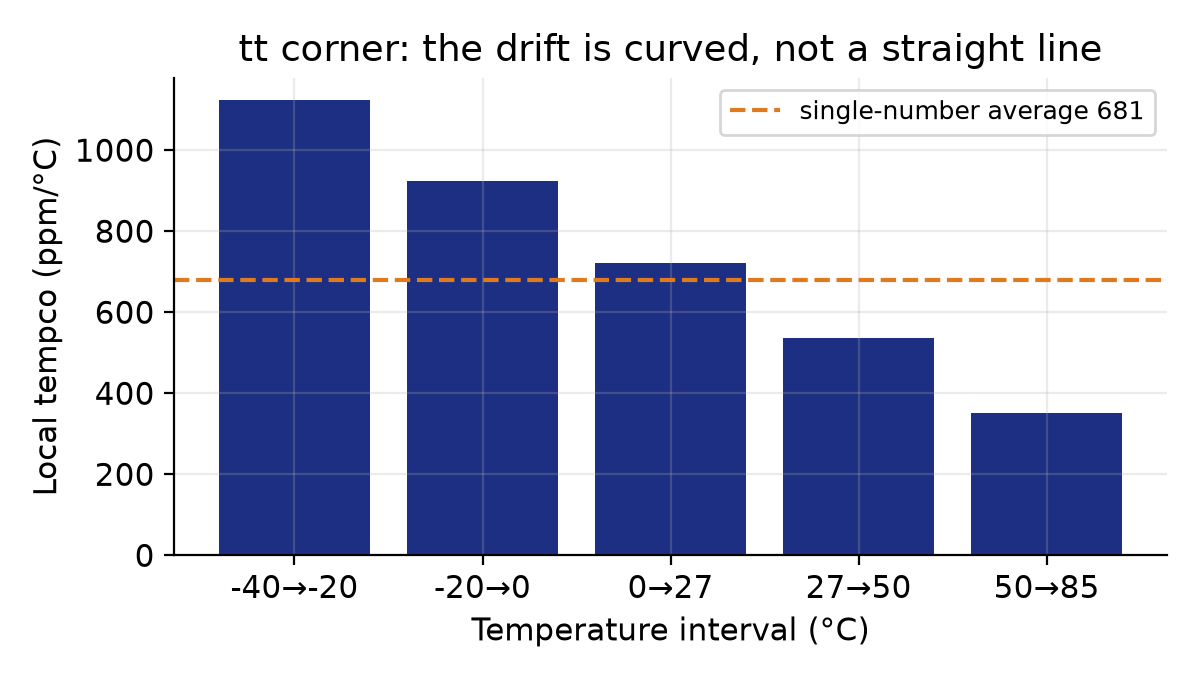
\includegraphics[width=0.6\linewidth]{tt_local.png}\end{center}
The tt tempco measured over each temperature interval falls from 1123 ppm/\textdegree C (cold) to 352 (hot). A straight line (1st order) can only match the average slope of 681 ppm/\textdegree C, so it leaves a bowed residual. Adding $k_2(T-27)^2$ matches that bow.

%=====================================================================
\section{The compensation network}
\begin{center}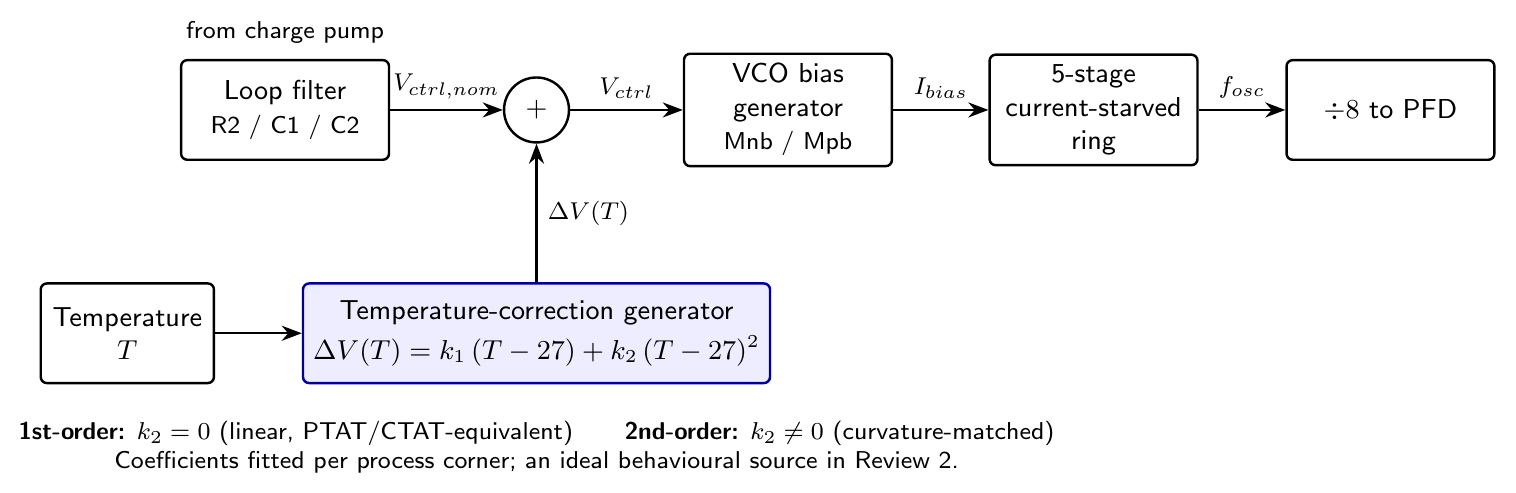
\includegraphics[width=0.9\linewidth]{compensation_arch.png}\end{center}
\[ V_{ctrl,eff} = V_{ctrl,nom} + k_1(T-27) + k_2(T-27)^2 \]
\begin{itemize}
\item \textbf{Implementation:} an ideal behavioural voltage source (an ngspice B-source) that reads the simulator temperature. \textbf{It is not transistors yet.} In silicon, this role is played by a PTAT/CTAT current generator.
\item \textbf{$k_1$ (analytical):} from the slope of the fitted $f(T)$ divided by $K_{VCO}$. Because the frequency rises with $T$, $k_1$ is negative.
\item \textbf{$k_2$, first attempt (naive):} derived from the curvature of the fit. It \emph{over-corrected} the cold end (+4.13\% at $-40$ \textdegree C, and a 4.49\% span, worse than 1st order's 3.05\%). The cause: it assumed $K_{VCO}$ is constant, which it is not.
\item \textbf{$k_2$, refined:} refit against the \emph{measured} residual left after 1st-order compensation. This step needed no extra simulation. At tt: $k_1=-1.320\times10^{-4}$ V/\textdegree C and $k_2=2.891\times10^{-7}$ V/\textdegree C$^2$.
\item \textbf{Per corner:} $k_1$ and $k_2$ are refit separately at every corner. In silicon this corresponds to a per-corner trim.
\end{itemize}

\subsection{Results at tt}
\begin{center}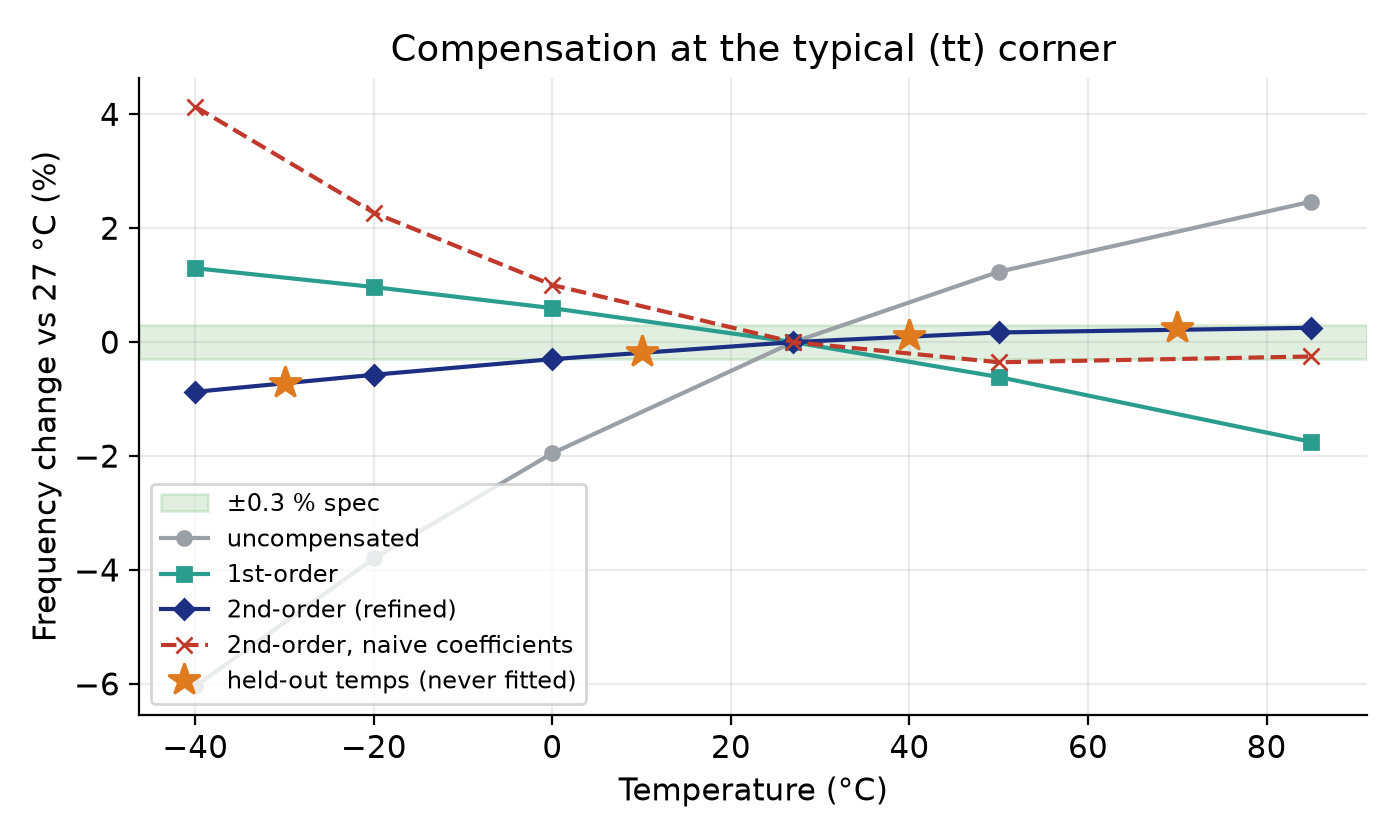
\includegraphics[width=0.72\linewidth]{comp_tt.png}\end{center}
\begin{itemize}
\item The span goes from 8.51\% (uncompensated) to 3.05\% (1st order) to 1.12\% (2nd order), so $C = 8.51/1.12 = 7.57\times$.
\item The maximum $|$deviation$|$ after 2nd order is 0.87\%, which does \textbf{not} meet $\pm$0.3\%.
\item \textbf{Held-out check (the orange points):} $-30$, 10, 40 and 70 \textdegree C were never used in fitting, and all of them fall inside the fitted envelope. This is our guard against overfitting 6 points with a 2-coefficient curve.
\end{itemize}

\subsection{Results at every corner}
\begin{center}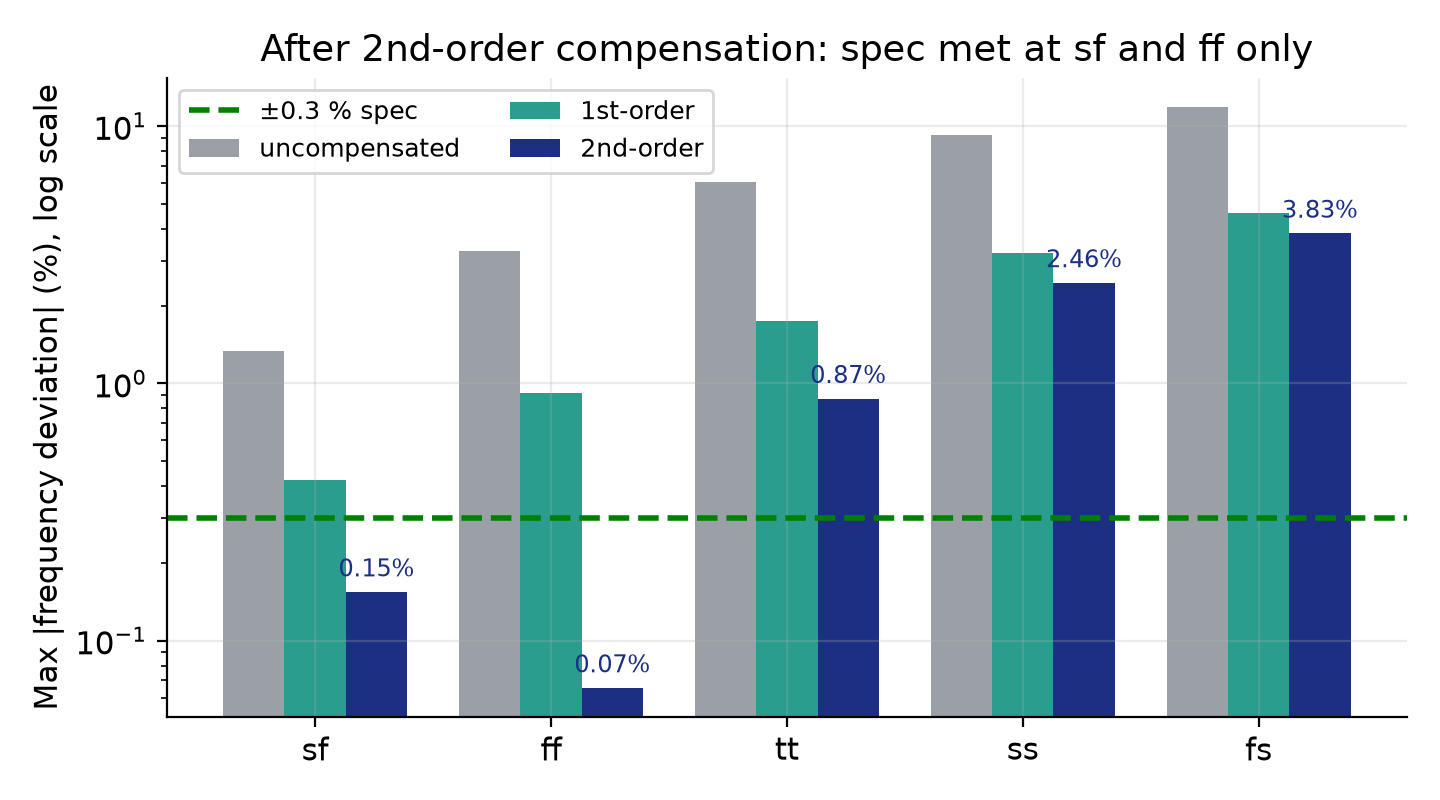
\includegraphics[width=0.72\linewidth]{comp_corners.png}\end{center}
\begin{center}
\begin{tabular}{lrrrrrl}\toprule
Corner & Baseline & 1st order & 2nd order & $C$ (2nd) & max$|$dev$|$ & Meets $\pm$0.3\%?\\\midrule
ff & 4.15\% & 1.06\% & 0.10\% & 40.3$\times$ & 0.07\% & \textcolor{ok}{yes}\\
sf & 1.48\% & 0.42\% & 0.24\% & 6.1$\times$ & 0.15\% & \textcolor{ok}{yes}\\
tt & 8.51\% & 3.05\% & 1.12\% & 7.6$\times$ & 0.87\% & \textcolor{warn}{no}\\
ss & 13.37\% & 6.37\% & 3.32\% & 4.0$\times$ & 2.46\% & \textcolor{warn}{no}\\
fs & 17.49\% & 9.13\% & 5.31\% & 3.3$\times$ & 3.83\% & \textcolor{warn}{no}\\\bottomrule
\end{tabular}
\end{center}
\noindent Every corner improves at both stages. \textbf{Span} means max $-$ min frequency over $-40$ to 85 \textdegree C, as a percentage of $f_{27}$. $C$ ranges over 12$\times$ across corners, which is why the project charter defines $C$ per corner and not as one number.

%=====================================================================
\section{Monte Carlo and the statistics}
\begin{center}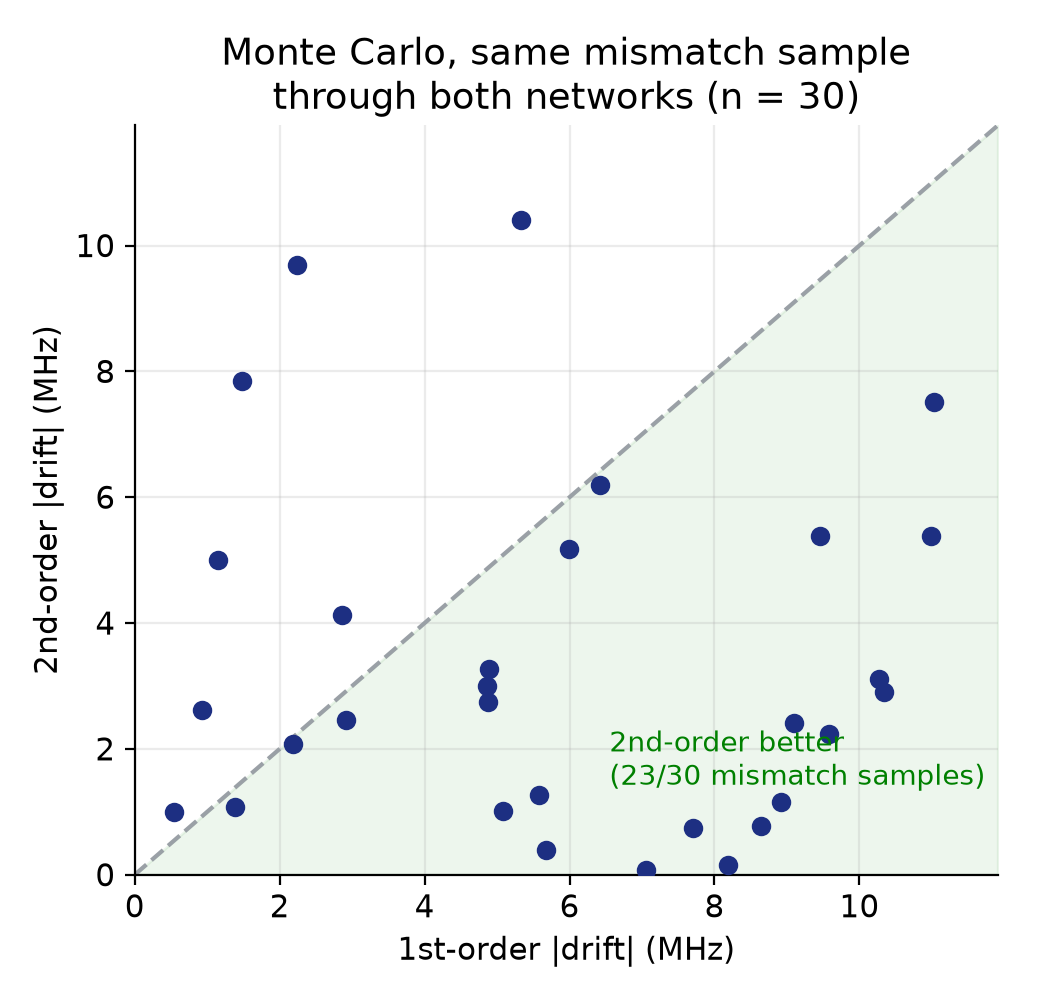
\includegraphics[width=0.42\linewidth]{mc_paired.png}\hfill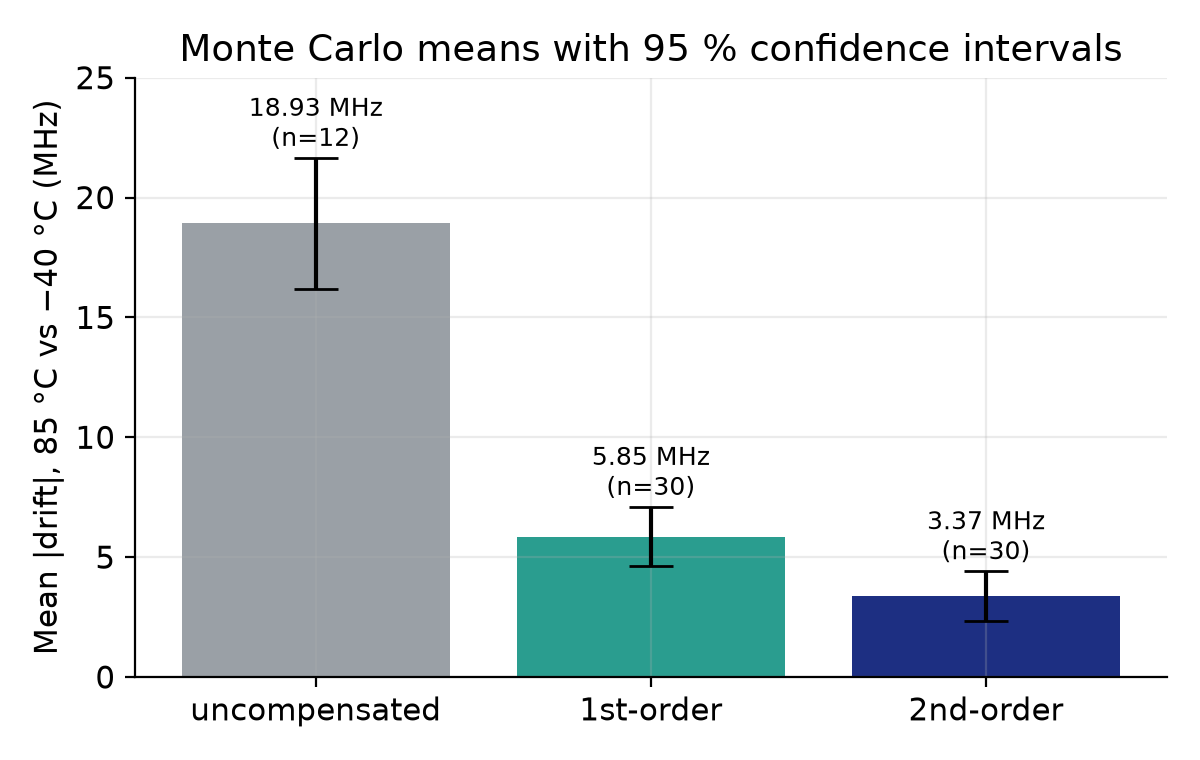
\includegraphics[width=0.54\linewidth]{mc_means.png}\end{center}
\begin{itemize}
\item \textbf{Setup:} tt corner with sky130's mismatch models switched on (\texttt{mc\_mm\_switch=1}). Each \emph{seed} is one virtual chip with random transistor mismatch.
\item \textbf{Metric:} $|$drift$|$ $= |f_{85}-f_{-40}|$ in MHz.
\item \textbf{Paired design:} the \emph{same} seed runs through both the 1st- and 2nd-order networks, so chip-to-chip variation cancels out of the comparison.
\item \textbf{Results:} mean $|$drift$|$ is 18.93 MHz uncompensated (n=12), 5.85 MHz for 1st order (n=30) and 3.37 MHz for 2nd order (n=30).
\item \textbf{2nd vs 1st:} a reduction of 2.48 MHz, 95\% CI [0.81, 4.15]. The paired t-test and the Wilcoxon signed-rank test are both significant, and 2nd order wins in 23 of 30 seeds.
\item \textbf{Two tests:} the t-test assumes normality; Wilcoxon does not. Both agreeing makes the result robust. Both are hand-implemented in \texttt{scripts/stats.py} (there is no scipy in this environment) and self-tested.
\end{itemize}
\begin{careful}
\textbf{The correction we made ourselves (own it, it is a strength).} The first analysis compared \emph{signed} drift. First order over-corrects (its drift is negative, $-5.7$ MHz) while second order under-corrects slightly ($+2.3$ MHz). Comparing signed values therefore made the difference look large simply because the sign flipped. The right quantity is $|$drift$|$. On $|$drift$|$ at n=12 the difference was \emph{not} significant, so we raised n to 30, and that is what earns the claim. This is recorded in \texttt{docs/stats\_methodology.md} and in the project charter's decision log.
\end{careful}

%=====================================================================
\section{Closed loop and the cold-start fix}
\begin{center}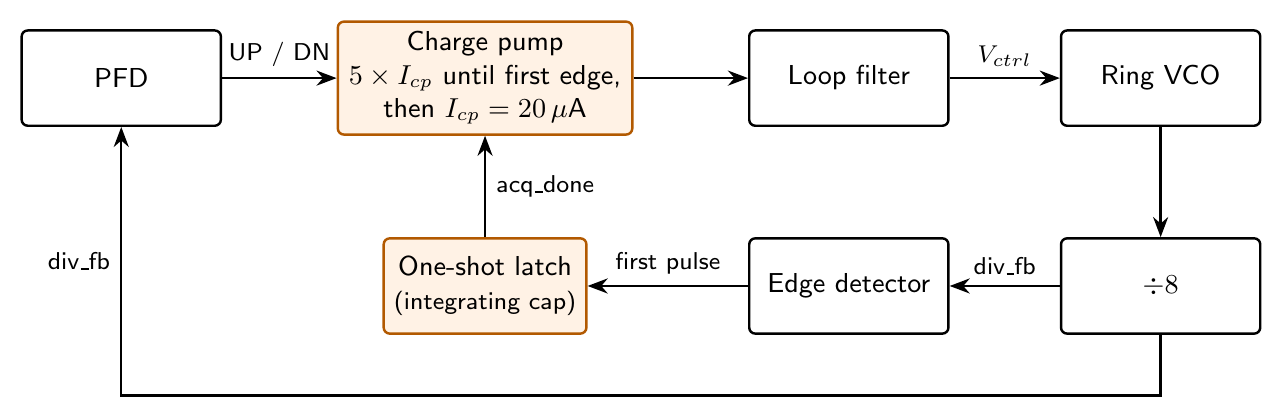
\includegraphics[width=0.66\linewidth]{acq_boost.png}\end{center}
\begin{center}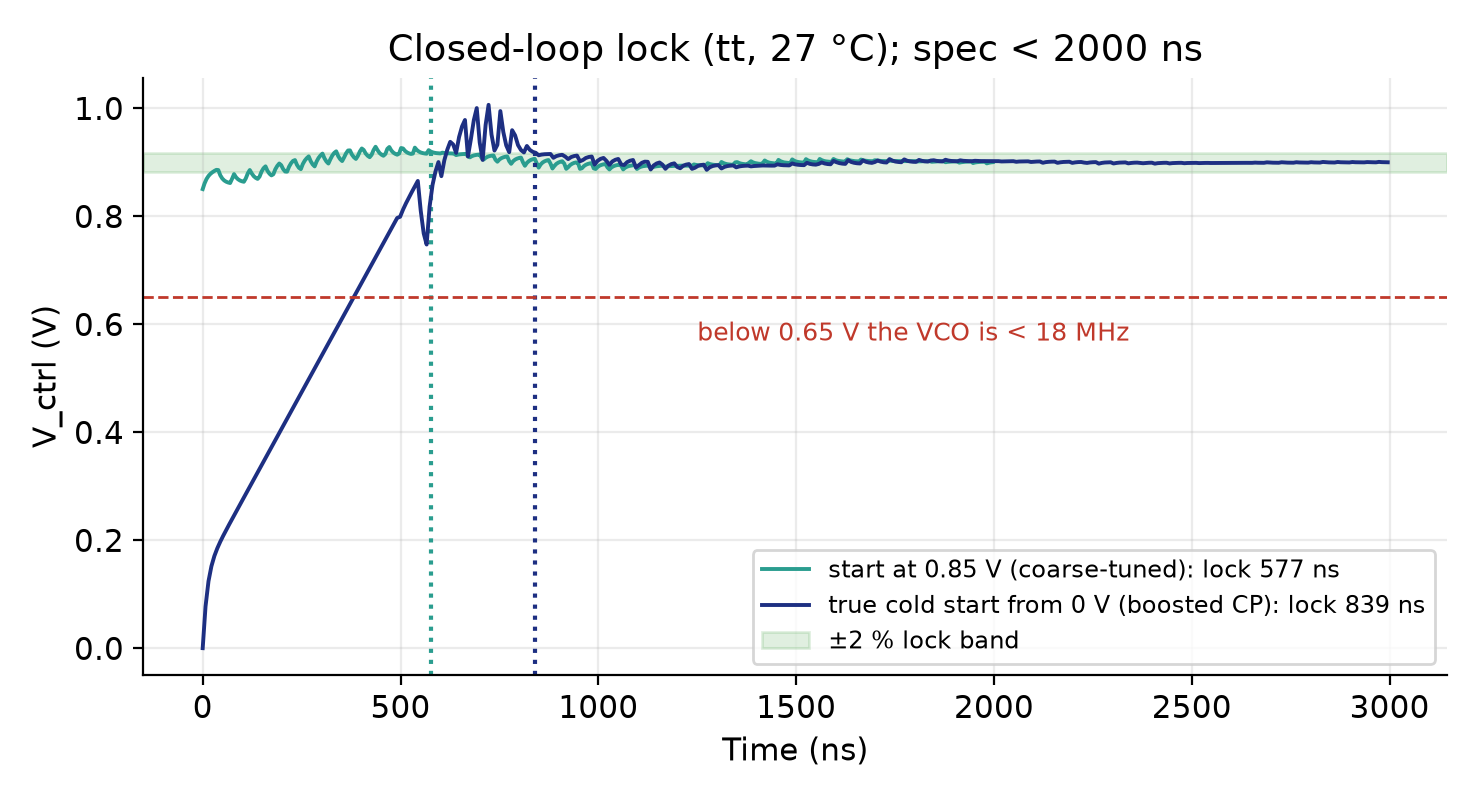
\includegraphics[width=0.7\linewidth]{lock.png}\end{center}
\begin{itemize}
\item \textbf{The problem:} at 0 V the VCO is below its 0.63 V oscillation floor, so it produces no edges. The divider stays silent and the PFD sees only the reference. Pumping up at 20 $\mu$A is slow, and there is a risk of a dead zone.
\item \textbf{The fix:} the charge pump runs at $5\times I_{cp}$ until the divider produces its first edge. An edge detector feeding a one-shot latch (an integrating capacitor charged by a B-source, not a digital latch with an unknown initial state) then drops it back to 20 $\mu$A for normal, stable tracking.
\item \textbf{Result:} lock in \textbf{839 ns} from a true 0 V start, and 577 ns from a coarse-tuned 0.85 V start. The spec is $<$2 $\mu$s; the analytical model predicted about 450 ns.
\item \textbf{Lock definition:} $V_{ctrl}$ enters and stays within $\pm2\%$ of its final 0.9 V.
\item \textbf{The ringing around 600--800 ns on the cold-start curve} is the loop capturing phase after the fast pump-up. It settles well inside the spec. We have not separately attributed it to the boost switching off, so don't claim that.
\end{itemize}

%=====================================================================
\section{Methodology and research framing}
\begin{center}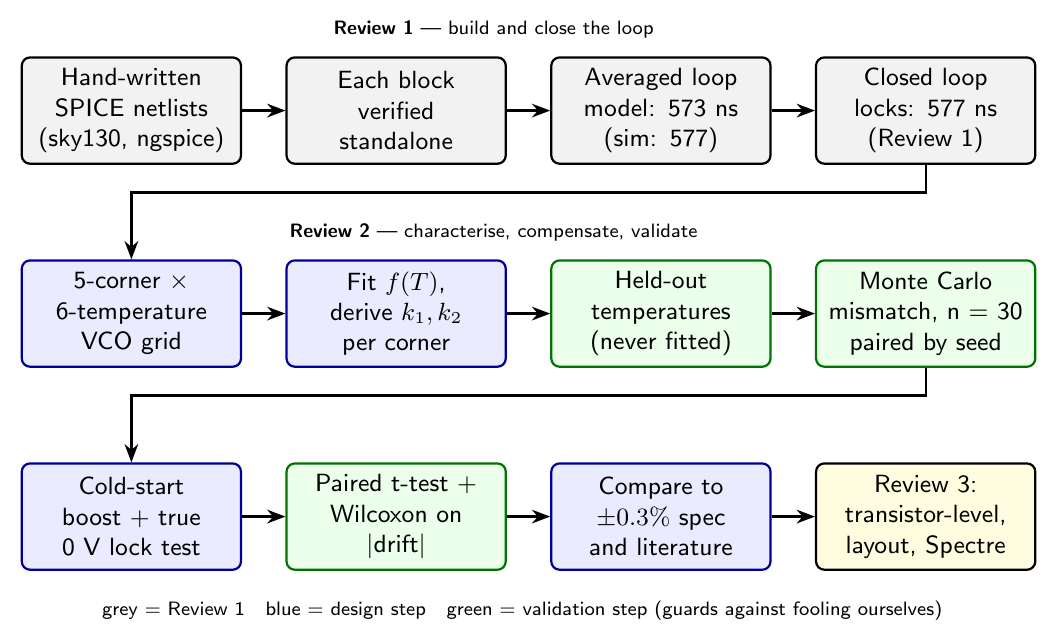
\includegraphics[width=\linewidth]{method_flow.png}\end{center}
\begin{itemize}
\item \textbf{Hypothesis H1 (the research question):} the error in a compensation network's residual grows as $\varepsilon_{res}\approx C\cdot\varepsilon_{raw}$. In words, the better you compensate, the more a small error in the drift \emph{measurement} (for example, from the open PDK's models versus a commercial one) is magnified in what remains. Testing it needs a second tool flow (Cadence Virtuoso/Spectre), which is \textbf{pending lab access}. The strength ($\alpha$) sweep we ran provides a range of $C$ values ready for that test; on its own it is \emph{not} the H1 test.
\item \textbf{Novelty (be precise):} US Patent 9,748,962 B2 (Infineon, 2017) already covers generic quadratic temperature compensation. We do \emph{not} claim quadratic compensation as new. Our claim is narrower: a quantified, statistically validated, per-corner study of it for a \emph{ring-VCO PLL, closed-loop, on an open PDK}.
\end{itemize}

%=====================================================================
\section{Slide-by-slide talking points}
\begin{enumerate}[label=\textbf{\arabic*.}]
\item \textbf{Title.} Names, guide, date.
\item \textbf{Introduction.} Problem, objectives, and what changed since Review 1: the 5-corner grid, the cold-start fix, and 2nd-order compensation.
\item[3--4.] \textbf{Literature.} 15 IEEE papers. The gap: nobody combines a compensated ring VCO, a closed-loop PLL, an open PDK and statistical validation.
\item[5.] \textbf{Architecture.} Walk the loop from REF to $\div8$, and name the two deliberate simplifications (ideal charge pump, latch-based PFD).
\item[6.] \textbf{VCO.} 669 MHz/V; the 0.63 V floor; 0.9 V gives 226 MHz.
\item[7.] \textbf{Compensation architecture.} $\Delta V(T)$ added before the bias generator; 1st vs 2nd order; per corner.
\item[8.] \textbf{Cold-start fix.} Problem, then the $5\times$ boost until the first edge.
\item[9.] \textbf{Methodology.} Grey is Review 1, blue is design, green is validation. The green steps are there to stop us fooling ourselves.
\item[10.] \textbf{Implementation.} The modules, the coefficient derivation, the hand-written statistics, and the B-source line.
\item[11.] \textbf{Results table.} 12.5$\times$ spread; the sf/fs insight.
\item[12.] \textbf{Drift chart.} Every corner is outside $\pm$0.3\%; fs is the worst.
\item[13.] \textbf{Curvature.} The bars would be equal if the drift were linear; they fall 3.2$\times$, which justifies $k_2$.
\item[14.] \textbf{Per-corner table.} Everything improves; the spec is met at ff and sf only.
\item[15.] \textbf{tt compensation chart.} 8.51 $\to$ 1.12\%; the naive curve (red dashed) failed; the held-out points pass.
\item[16.] \textbf{Per-corner chart.} Log scale; the green line is the spec. Say plainly: ``not met at tt, ss or fs''.
\item[17.] \textbf{Closed-loop table.} 577 / 839 ns; the two Review 1 bugs.
\item[18.] \textbf{Lock chart.} Point at the 0.63 V floor and at the boost carrying the voltage through it.
\item[19.] \textbf{MC and benchmark table.} Comparable to published work, but ours is simulation and theirs is silicon.
\item[20.] \textbf{MC charts.} Points below the diagonal are chips where 2nd order won (23/30).
\item[21.] \textbf{At a glance.} Eight numbers.
\item[22.] \textbf{Challenges and remaining work.} The honest list, then Review 3.
\end{enumerate}

%=====================================================================
\section{Numbers to memorise}
\begin{center}
\begin{tabular}{ll}\toprule
Reference / output / N & 28.275 MHz / $\approx$226 MHz / 8\\
Loop filter, $I_{cp}$ & $R_2$ 1.7 k$\Omega$, $C_1$ 68 pF, $C_2$ 6.8 pF; 20 $\mu$A\\
$K_{VCO}$ (tt, 0.9 V) & 669 MHz/V; floor $\approx$0.63 V\\
Tempco sf/ff/tt/ss/fs & 112 / 332 / 681 / 1070 / 1399 ppm/\textdegree C (12.5$\times$)\\
tt span: base $\to$ 1st $\to$ 2nd & 8.51 $\to$ 3.05 $\to$ 1.12\%, $C=7.57\times$\\
tt max$|$dev$|$ (2nd) & 0.87\% (spec $\pm$0.3\%)\\
Spec met at & ff (0.07\%), sf (0.15\%)\\
MC mean $|$drift$|$ & 18.93 / 5.85 / 3.37 MHz\\
2nd vs 1st & $-2.48$ MHz, CI [0.81, 4.15], 23/30 seeds\\
Lock & 577 ns (0.85 V start), 839 ns (0 V), spec $<$2 $\mu$s\\
Temperatures & $-40$, $-20$, 0, 27, 50, 85; held-out $-30$, 10, 40, 70\\\bottomrule
\end{tabular}
\end{center}

%=====================================================================
\section{Likely questions and answers}
\qa{Your spec is $\pm$0.3\% and you only meet it at 2 of 5 corners. Isn't that a failure?}{It is a gap, and we say so on the slide. The correction is currently a fixed curve per corner. Closing the gap at tt/ss/fs needs a transistor-level network whose PTAT slope itself tracks process, and/or a trim. That is Review 3 work. What Review 2 establishes is how large the problem is, and that 2nd order beats 1st order with statistical confidence.}

\qa{The compensation is an ideal source. How real is this?}{It is a behavioural model, as is standard at this stage: it tells us \emph{what} correction voltage is needed. In silicon it would be a PTAT/CTAT current generator driving a resistor; a quadratic term can come from combining PTAT and a squared term (for example, a translinear stage). Building that at transistor level is Review 3.}

\qa{Why a ring VCO and not an LC oscillator?}{A ring is small, has a wide tuning range and needs no inductor, which suits a digital-friendly open PDK. Its disadvantage is exactly what we study: large temperature sensitivity (and worse phase noise).}

\qa{Why is there no phase noise or jitter result?}{Out of scope for Review 2, which focuses on temperature. A transient-noise or PSS-style analysis in ngspice is limited; this would be part of the Spectre arm.}

\qa{Why sky130 and ngspice?}{They are fully open, so the work is reproducible by anyone; the PDK is pinned by commit via volare. The trade-off is less mature models, which is exactly why H1 plans a Spectre cross-check.}

\qa{How do you know you didn't overfit? Six points, two coefficients.}{Four held-out temperatures that were never used in fitting, at every corner, all fall inside the fitted envelope. The Monte Carlo analysis also tests the same coefficients on 30 mismatched chips.}

\qa{Why was the naive $k_2$ wrong?}{It assumed $K_{VCO}$ is constant with temperature and voltage. It is not: the tuning curve is nonlinear. Refitting against the measured 1st-order residual absorbs that.}

\qa{Why is Monte Carlo only at tt, and why is the baseline n=12?}{Compute time. The baseline effect is huge (12/12 seeds, reduction CI [9.98, 15.57] MHz), so n=12 is already decisive there. The 1st-vs-2nd difference is small, so it needed n=30.}

\qa{What was the statistics error?}{We compared signed drift, but 1st order over-corrects and 2nd order under-corrects slightly, so the sign flip inflated the difference. We switched to $|$drift$|$, found it not significant at n=12, and re-ran at n=30, where it is significant. It is documented in the repo.}

\qa{What is new, given the Infineon patent?}{Quadratic compensation itself is not new. What is new is the quantified, per-corner, statistically validated study on a ring-VCO PLL in closed loop on an open PDK, and the H1 error-amplification question.}

\qa{Why does the frequency increase with temperature?}{Most likely because, at our bias, the fall in threshold voltage with temperature outweighs the fall in mobility, so the starving current rises. This is an interpretation, not something we isolated in simulation.}

\qa{What does the acquisition boost do to stability?}{It is only active before the first divider edge, while the loop is still open. After that, the charge pump runs at the nominal 20 $\mu$A for which the loop was designed, so stability during tracking is unchanged.}

\qa{Why a latch-based PFD?}{A resettable-D-flip-flop PFD needs a clean asynchronous reset. In our hand-built cells, that reset fought the latch's bistable feedback. Edge detectors plus NOR SR-latches were reliable, and the PFD was verified standalone in Review 1.}

\qa{What is left for Review 3?}{A transistor-level charge pump and compensation network; layout in Magic with DRC and LVS (netgen); post-layout simulation; and the Spectre arm with the H1 regression. The deadline is 28.10.2026.}

%=====================================================================
\section{Glossary}
\begin{description}[style=nextline,leftmargin=1.2em,itemsep=1pt]
\item[Process corner] The five sets of device models: tt (typical), ff/ss (both fast/slow), sf/fs (NMOS slow + PMOS fast, and the reverse).
\item[Tempco] The fractional frequency change per \textdegree C, in ppm/\textdegree C.
\item[Span] Max $-$ min frequency over temperature, as a percentage of the 27 \textdegree C frequency.
\item[Compensation ratio $C$] Baseline span divided by compensated span. Bigger is better.
\item[PTAT / CTAT] Proportional / complementary to absolute temperature: bias sources that rise or fall linearly with $T$.
\item[$K_{VCO}$] The VCO gain, $df/dV_{ctrl}$.
\item[Lock time] Time until $V_{ctrl}$ stays within $\pm2\%$ of its final value.
\item[Seed] One Monte Carlo sample, i.e.\ one random mismatch instance (a virtual chip).
\item[Paired t-test / Wilcoxon] Tests on per-seed differences. The t-test assumes normality; Wilcoxon uses ranks and does not.
\item[95\% CI] The range that contains the true mean difference with 95\% confidence. If it excludes 0, the effect is significant.
\item[Held-out] Data points kept out of the fit and used only to test it.
\end{description}
\end{document}
